\documentclass[compress]{beamer}
\usepackage{ifthen,verbatim}

\newcommand{\isnote}{}
\xdefinecolor{lightyellow}{rgb}{1.,1.,0.25}
\xdefinecolor{darkblue}{rgb}{0.1,0.1,0.7}

%% Uncomment this to get annotations
%% \def\notes{\addtocounter{page}{-1}
%%            \renewcommand{\isnote}{*}
%% 	   \beamertemplateshadingbackground{lightyellow}{white}
%%            \begin{frame}
%%            \frametitle{Notes for the previous page (page \insertpagenumber)}
%%            \itemize}
%% \def\endnotes{\enditemize
%% 	      \end{frame}
%%               \beamertemplateshadingbackground{white}{white}
%%               \renewcommand{\isnote}{}}

%% Uncomment this to not get annotations
\def\notes{\comment}
\def\endnotes{\endcomment}

\setbeamertemplate{navigation symbols}{}
\setbeamertemplate{headline}{\mbox{ } \hfill
\begin{minipage}{5.5 cm}
\vspace{-0.75 cm} \small
\end{minipage} \hfill
\begin{minipage}{4.5 cm}
\vspace{-0.75 cm} \small
\begin{flushright}
\ifthenelse{\equal{\insertpagenumber}{1}}{}{Jim Pivarski \hspace{0.2 cm} \insertpagenumber\isnote/\pageref{numpages}}
\end{flushright}
\end{minipage}\mbox{\hspace{0.2 cm}}\includegraphics[height=1 cm]{../cmslogo} \hspace{0.1 cm} \includegraphics[height=1 cm]{../tamulogo} \hspace{0.01 cm} \vspace{-1.05 cm}}

\begin{document}
\begin{frame}
\vfill
\begin{center}
\textcolor{darkblue}{\Large 50~pb$^{-1}$ Misalignment Scenario}

\vfill
\begin{columns}
\column{0.3\linewidth}
\begin{center}
\large
\textcolor{darkblue}{Jim Pivarski}
\end{center}
\end{columns}

\begin{columns}
\column{0.3\linewidth}
\begin{center}
\scriptsize
{\it Texas A\&M University}
\end{center}
\end{columns}

\vfill
18 August, 2009

\end{center}
\end{frame}

%% \begin{notes}
%% \item This is the annotated version of my talk.
%% \item If you want the version that I am presenting, download the one
%% labeled ``slides'' on Indico (or just ignore these yellow pages).
%% \item The annotated version is provided for extra detail and a written
%% record of comments that I intend to make orally.
%% \item Yellow notes refer to the content on the {\it previous} page.
%% \item All other slides are identical for the two versions.
%% \end{notes}

\small

\begin{frame}
\frametitle{Motivation}
\begin{itemize}
\item STARTUP scenarios are based on CRAFT experience

\vspace{0.1 cm}
\begin{itemize}\setlength{\itemsep}{0.25 cm}
\item tracker STARTUP misalignment: constructed from earlier scenarios to yield data-driven resolutions seen in CRAFT
\item muon STARTUP misalignment: as much as possible, the same distributions as CRAFT (e.g.~no alignment in wheel $\pm$2)
\end{itemize}

\item It would be pessimistic to assume that alignment will not improve with collisions in 2010, especially ``unaligned'' chambers
\end{itemize}

\vfill
\hspace{-0.83 cm} \textcolor{darkblue}{\Large Definition of 50~pb$^{-1}$ scenario}

\vspace{0.2 cm}
\begin{itemize}
\item tracker misalignment: same as STARTUP
\item muon misalignment: result of MC exercise, using tracker misalignment and latest MuonAlignmentFromReference
\end{itemize}
\end{frame}

\begin{frame}
\frametitle{STARTUP tracker misalignment}

\begin{itemize}\setlength{\itemsep}{0.1 cm}
\item Definition:
\begin{itemize}
\item TIB and TOB: same as 100~pb$^{-1}$ scenario
\item Pixel endcap: same as SurveyLASOnly (i.e.~no tracks)
\item everything else: same as 10~pb$^{-1}$ scenario
\end{itemize}

\item Randomly-generated with hierarchial errors

\item Roughly $\phi$-symmetric: unlike cosmic ray alignment but like early collisions alignment
\end{itemize}

\begin{columns}
\column{0.6\linewidth}
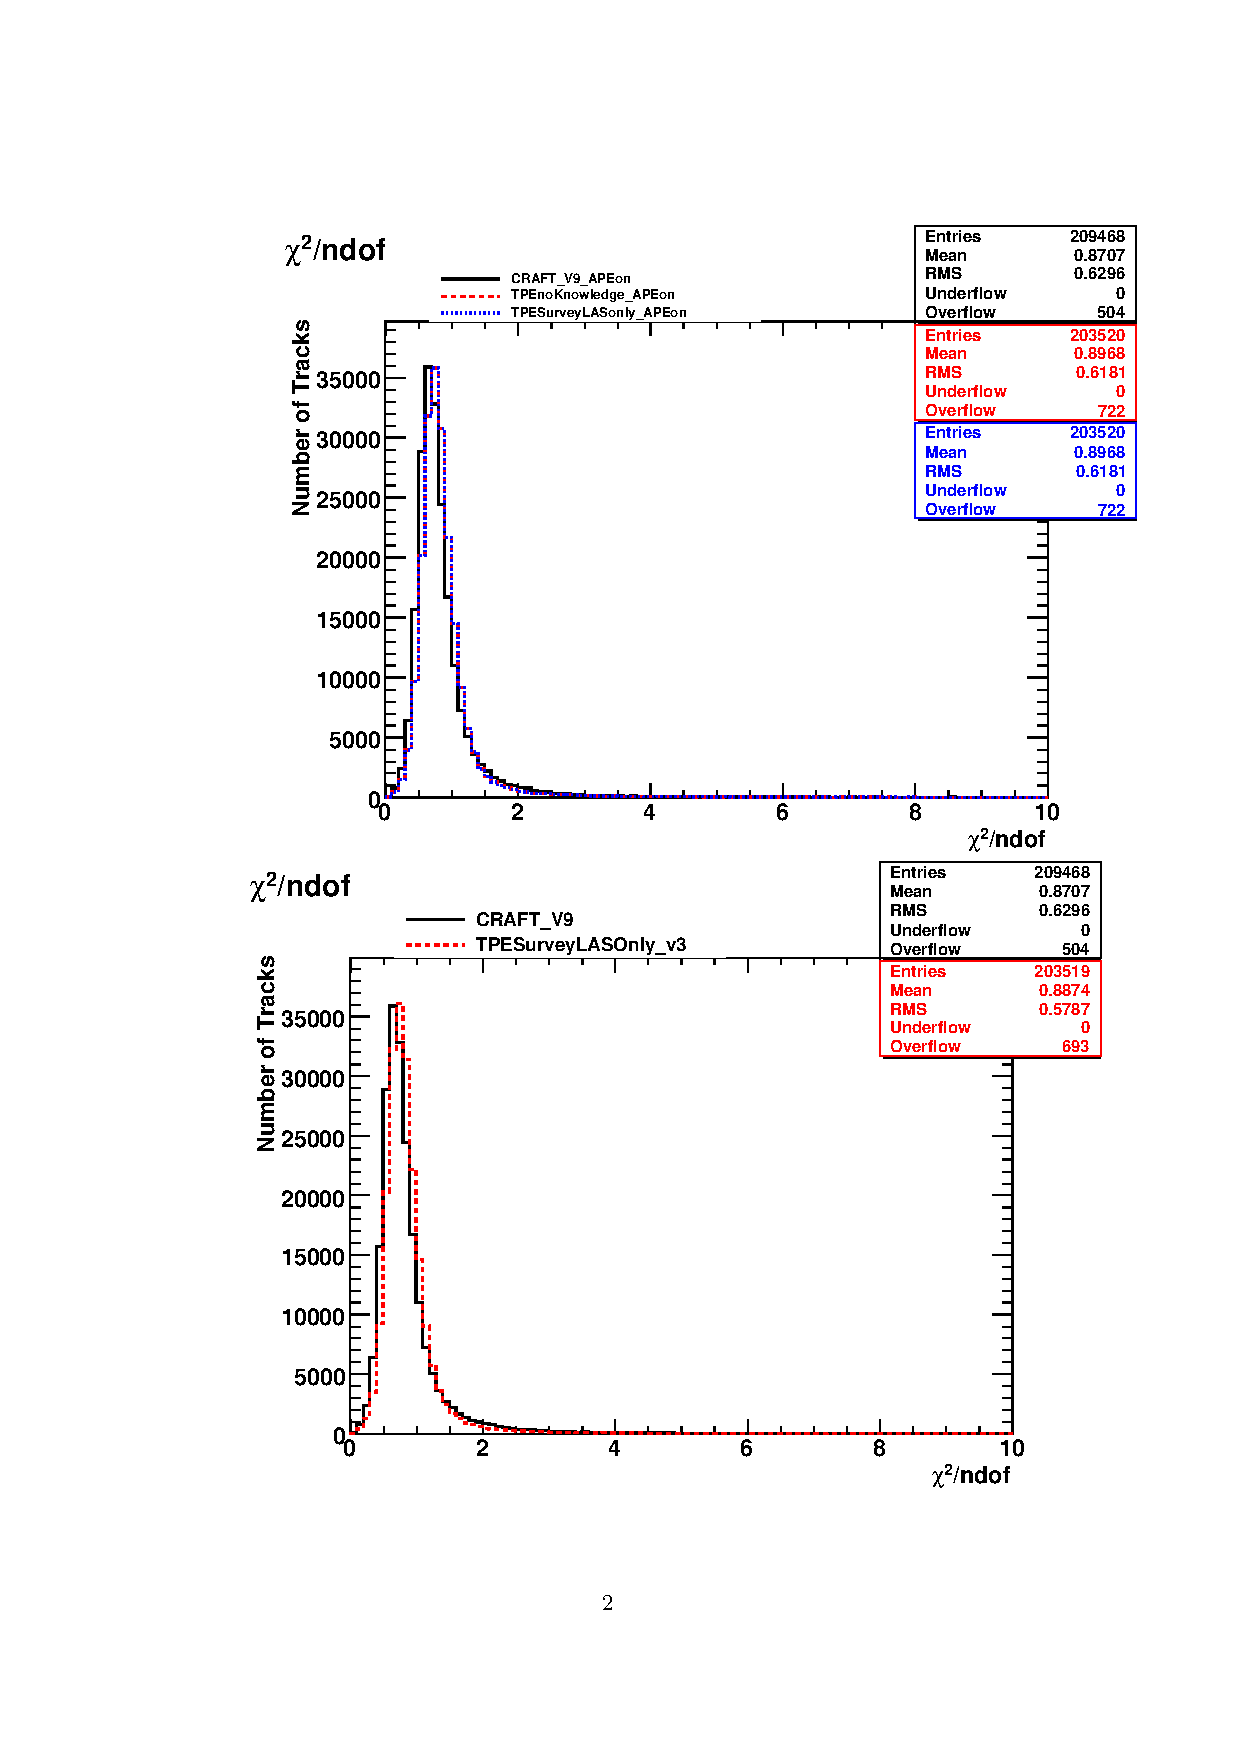
\includegraphics[width=\linewidth]{tracker_chi2.pdf}
\column{0.4\linewidth}

Jula Draeger, Gero Fluke

\vspace{0.4 cm}
Real-data CRAFT alignment yields better $\chi^2$ \\ {\it (in modules sampled by vertical cosmic rays)}

\vspace{0.4 cm}
Similar picture from residuals, DMR, and Nhan's split cosmics tests
\end{columns}
\end{frame}

\begin{frame}
\frametitle{50~pb$^{-1}$ muon misalignment}

\begin{itemize}
\item Procedure \mbox{(using MuonAlignmentFromReference on simulated data)\hspace{-1 cm}}
\begin{enumerate}
\item start with no-tracks random misalignment
\item align as many chambers as possible (mostly central barrel) with \textcolor{darkblue}{$p_T > 100$~GeV cosmic rays} in 6 degrees of freedom
\item re-align all chambers with \textcolor{darkblue}{$p_T > 20$~GeV collisions} with $\delta_z$ fixed
\end{enumerate}

\item Why?
\begin{itemize}
\item we use average of separate $\mu^+$ and $\mu^-$ alignments
  (``two-bin method'') to reduce sensitivity to $dE/dx$ and
  $\vec{B}(\vec{x})$ errors
\item this method works for all parameters except $\delta_z$:
\begin{center} \includegraphics[width=0.7\linewidth]{explanation_of_z.pdf} \end{center}

\item alternative is to align at very high energies ($p_T > 100$~GeV), where $dE/dx$ and
  $\vec{B}(\vec{x})$ don't matter

\item such high-energy muons are only available in cosmic rays
\end{itemize}
\end{itemize}
\end{frame}

\begin{frame}
\frametitle{Results: cosmic ray pass}

\begin{itemize}
\item Only showing aligned chambers
\item Final product includes tracker misalignment (yellow)
\end{itemize}

\includegraphics[height=\linewidth, angle=90]{scenario_cosmics.pdf}
\end{frame}

\begin{frame}
\frametitle{Results: collisions pass}

\begin{itemize}
\item Showing all chambers (except one fit failure), \mbox{only aligned parameters\hspace{-1 cm}}
\begin{itemize}
\item barrel stations 1--3: all but $\delta_z$ (but showing inherited $\delta_z$)
\item barrel station 4: only $\delta_x$, $\delta_{\phi_y}$, $\delta_{\phi_z}$ (no $\Delta y$)
\item CSCs: only $\delta_x$, $\delta_{\phi_y}$, $\delta_{\phi_z}$ (poor $\Delta y$)
\end{itemize}

\item Note 490~$\mu$m $\delta_x$ resolution and \mbox{low sensitivity to tracker misalignment\hspace{-1 cm}}
\end{itemize}

\includegraphics[height=\linewidth, angle=90]{scenario_cosmics_then_collisions.pdf}
\end{frame}

\begin{frame}
\frametitle{Dependence on tracker}

\vspace{0.2 cm}
\begin{columns}
\column{0.67\linewidth}
\begin{itemize}
\item \textcolor{darkblue}{Right:} CSA08 station~1 (best) resolution, with and without S156 tracker misal
\item \textcolor{darkblue}{Below:} 50~pb$^{-1}$ resolution for all chambers, with and without STARTUP tracker misal
\item \textcolor{darkblue}{Caution!} apples and oranges:
\begin{itemize}
\item S156 is the result of an algorithm, different correlations than random
\item S156 was a 10~pb$^{-1}$ exercise, but achieved unexpectedly high resolution
\end{itemize}
\end{itemize}

\begin{columns}
\column{0.4\linewidth}
\begin{itemize}
\item However, new \mbox{muon alignment\hspace{-0.5 cm}} algorithm seems to be less sensitive
\end{itemize}

\column{0.6\linewidth}

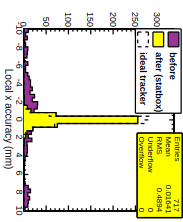
\includegraphics[height=\linewidth, angle=90]{scenario_cosmics_then_collisions_redrawn.pdf}
\end{columns}

\column{0.33\linewidth}
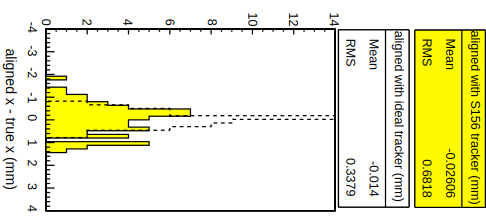
\includegraphics[height=\linewidth, angle=90]{muonalignment_MB1_dep_on_tracker_redrawn.pdf}
\end{columns}
\end{frame}

\begin{frame}
\frametitle{Unaligned degrees of freedom}

\begin{itemize}\setlength{\itemsep}{0.35 cm}
\item Station~4 DTs and all CSCs have little sensitivity to global $z$
  for basic read-out or geometrical reasons
\begin{itemize}
\item global $z$ component of their APEs $\to$ 1000~cm
\end{itemize}

\item In addition, ME1/3 chambers were fixed to initial misaligned
  positions due to errors (many fit failures)

\begin{itemize}
\item all components of their APEs $\to$ 1000~cm
\item (we should investigate, but it may be an old problem in the 22X MC)
\end{itemize}

\item All other APEs $\to$ 0

\item Important to use these AlignmentErrorRcds to mask out unaligned parameters
\end{itemize}
\end{frame}

%% \section*{First section}
%% \begin{frame}
%% \begin{center}
%% \Huge \textcolor{blue}{First section}
%% \end{center}
%% \end{frame}

\begin{frame}
\frametitle{Concluding remarks}

\begin{itemize}\setlength{\itemsep}{0.35 cm}
\item ``Intermediate'' (between STARTUP and DESIGN) scenario useful
  for early physics analyses that depend on muon alignment
\item Running the alignment algorithm itself matches muon chamber
  positions to a given tracker misalignment scenario
\item Where to find the muon alignment (4 records, including APEs):

{\tiny \tt
/afs/cern.ch/user/p/pivarski/public/MuonAlignmentRcd\_cosmics-50pb-1-noME13\_3XY\_v1.db
/afs/cern.ch/user/p/pivarski/public/MuonAlignmentRcd\_cosmics-50pb-1-noME13\_22X\_v1.db
/afs/cern.ch/user/p/pivarski/public/MuonAlignmentRcd\_cosmics-50pb-1-noME13\_v1.xml
}

\item See backup for \_cfg.py 22X snippet
\end{itemize}

\label{numpages}
\end{frame}

\begin{frame}
\frametitle{How to use it in 22X}
\tiny \tt
process.load("Configuration.StandardSequences.FrontierConditions\_GlobalTag\_noesprefer\_cff") \\
process.GlobalTag.globaltag = cms.string("CRAFT\_ALL\_V12::All") \\
process.es\_prefer\_cscBadChambers = cms.ESPrefer("PoolDBESSource", "cscBadChambers") \\
del process.DTFakeVDriftESProducer \\
\mbox{ } \\
from CondCore.DBCommon.CondDBSetup\_cfi import * \\
process.MuonAlignmentInputSQLite = cms.ESSource("PoolDBESSource", \\
\hspace{1 cm}CondDBSetup, \\
\hspace{1 cm}connect = cms.string( \\
"sqlite\_file:/afs/cern.ch/user/p/pivarski/public/MuonAlignmentRcd\_cosmics-50pb-1-noME13\_22X\_v1.db"), \\
\hspace{1.5 cm}toGet = cms.VPSet(cms.PSet(record = cms.string("DTAlignmentRcd"), \\
\hspace{2.5 cm}tag = cms.string("DTAlignmentRcd")), \\
\hspace{2 cm}cms.PSet(record = cms.string("DTAlignmentErrorRcd"), \\
\hspace{2.5 cm}tag = cms.string("DTAlignmentErrorRcd")), \\
\hspace{2 cm}cms.PSet(record = cms.string("CSCAlignmentRcd"), \\
\hspace{2.5 cm}tag = cms.string("CSCAlignmentRcd")), \\
\hspace{2 cm}cms.PSet(record = cms.string("CSCAlignmentErrorRcd"), \\
\hspace{2.5 cm}tag = cms.string("CSCAlignmentErrorRcd")))) \\
process.TrackerAlignmentInputDB = cms.ESSource("PoolDBESSource", \\
\hspace{1 cm}CondDBSetup, \\
\hspace{1 cm}connect = cms.string("frontier://FrontierProd/CMS\_COND\_21X\_ALIGNMENT"), \\
\hspace{1.5 cm}toGet = cms.VPSet(cms.PSet(record = cms.string("TrackerAlignmentRcd"), \\
\hspace{2.5 cm}tag = cms.string("TrackerCRAFTScenario22X\_v3\_mc")), \\
\hspace{2 cm}cms.PSet(record = cms.string("TrackerAlignmentErrorRcd"), \\
\hspace{2.5 cm}tag = cms.string("Tracker\_GeometryErr\_v3\_offline")))) \\
\mbox{process.es\_prefer\_MuonAlignmentInputSQLite = cms.ESPrefer("PoolDBESSource", "MuonAlignmentInputSQLite")\hspace{-2 cm}} \\
\mbox{process.es\_prefer\_TrackerAlignmentInputDB = cms.ESPrefer("PoolDBESSource", "TrackerAlignmentInputDB")\hspace{-2 cm}}
\end{frame}

\begin{frame}
\frametitle{Alternative}
\framesubtitle{The following has been reported to work better}
\tiny \tt
process.load("Configuration.StandardSequences.FrontierConditions\_GlobalTag\_cff") \\
process.GlobalTag.globaltag = cms.string("CRAFT\_ALL\_V12::All") \\
del process.es\_prefer\_GlobalTag \\
del process.DTFakeVDriftESProducer \\
\mbox{ } \\
from CondCore.DBCommon.CondDBSetup\_cfi import * \\
process.MuonAlignmentInputSQLite = cms.ESSource("PoolDBESSource", \\
\hspace{1 cm}CondDBSetup, \\
\hspace{1 cm}connect = cms.string( \\
"sqlite\_file:/afs/cern.ch/user/p/pivarski/public/MuonAlignmentRcd\_cosmics-50pb-1-noME13\_22X\_v1.db"), \\
\hspace{1.5 cm}toGet = cms.VPSet(cms.PSet(record = cms.string("DTAlignmentRcd"), \\
\hspace{2.5 cm}tag = cms.string("DTAlignmentRcd")), \\
\hspace{2 cm}cms.PSet(record = cms.string("DTAlignmentErrorRcd"), \\
\hspace{2.5 cm}tag = cms.string("DTAlignmentErrorRcd")), \\
\hspace{2 cm}cms.PSet(record = cms.string("CSCAlignmentRcd"), \\
\hspace{2.5 cm}tag = cms.string("CSCAlignmentRcd")), \\
\hspace{2 cm}cms.PSet(record = cms.string("CSCAlignmentErrorRcd"), \\
\hspace{2.5 cm}tag = cms.string("CSCAlignmentErrorRcd")))) \\
process.TrackerAlignmentInputDB = cms.ESSource("PoolDBESSource", \\
\hspace{1 cm}CondDBSetup, \\
\hspace{1 cm}connect = cms.string("frontier://FrontierProd/CMS\_COND\_21X\_ALIGNMENT"), \\
\hspace{1.5 cm}toGet = cms.VPSet(cms.PSet(record = cms.string("TrackerAlignmentRcd"), \\
\hspace{2.5 cm}tag = cms.string("TrackerCRAFTScenario22X\_v3\_mc")), \\
\hspace{2 cm}cms.PSet(record = cms.string("TrackerAlignmentErrorRcd"), \\
\hspace{2.5 cm}tag = cms.string("Tracker\_GeometryErr\_v3\_offline")))) \\
\mbox{process.es\_prefer\_MuonAlignmentInputSQLite = cms.ESPrefer("PoolDBESSource", "MuonAlignmentInputSQLite")\hspace{-2 cm}} \\
\mbox{process.es\_prefer\_TrackerAlignmentInputDB = cms.ESPrefer("PoolDBESSource", "TrackerAlignmentInputDB")\hspace{-2 cm}}
\end{frame}

\end{document}
